\documentclass{article}

\usepackage{amsmath,amssymb}
\usepackage{tikz}
\usepackage{xcolor}
\usepackage[left=2.1cm,right=3.1cm,bottom=3cm,footskip=0.75cm,headsep=0.5cm]{geometry}
\usepackage{enumerate}
\usepackage{enumitem}

\usepackage[utf8]{inputenc}

\renewcommand*{\arraystretch}{1.4}

\title{\textbf{Einführung in die Informatik, Übung 7}}
\author{\textsc{Henry Haustein}}
\date{}

\begin{document}
	\maketitle
	
	\section*{Aufgabe 7.1}
	
	\begin{enumerate}[label=(\alph*)]
		\item nein, $abba\notin L(\mathcal{A})$
		\item $w_1$: nein, Endpunkt $q_4$ \\
		$w_2$: nein, von $q_5$ kein Zweig mit $b$ \\
		$w_3$: ja, man bleibt bei $q_6$
	\end{enumerate}
	
	\section*{Aufgabe 7.2}
	
	\begin{enumerate}[label=(\alph*)]
		\item $\mathcal{A} = (\{q_0,q_1\},\Sigma,q_0,\Delta_a,\{q_0\})$, mit $\Delta_a$
		\begin{center}
			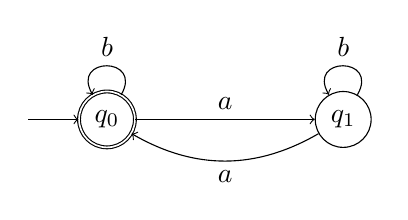
\begin{tikzpicture}
				\node[circle,draw=black, fill=white, double] (q0) at (0,0) {$q_0$};
				\node[circle,draw=black, fill=white] (q1) at (3,0) {$q_1$};
				
				\draw[->] (-1,0) -- (q0);
				\draw[->] (q0) to node[midway,above] {$a$} (q1);
				\draw[->] (q1) to[bend left=30] node[midway,below] {$a$} (q0);
				\draw[->,looseness=4] (q0) to[out=60,in=120] node[midway,above] {$b$} (q0);
				\draw[->,looseness=4] (q1) to[out=60,in=120] node[midway,above] {$b$} (q1);
			\end{tikzpicture}
		\end{center}
		\item $\mathcal{B}=(\{q_0,q_1,q_2,q_3\},\Sigma,q_0,\Delta_b,\{q_3\})$ mit $\Delta_b$
		\begin{center}
			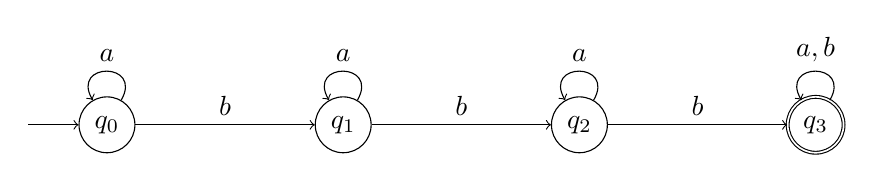
\begin{tikzpicture}
				\node[circle,draw=black, fill=white] (q0) at (0,0) {$q_0$};
				\node[circle,draw=black, fill=white] (q1) at (3,0) {$q_1$};
				\node[circle,draw=black, fill=white] (q2) at (6,0) {$q_2$};
				\node[circle,draw=black, fill=white,double] (q3) at (9,0) {$q_3$};
				
				\draw[->] (-1,0) -- (q0);
				\draw[->] (q0) to node[midway,above] {$b$} (q1);
				\draw[->] (q1) to node[midway,above] {$b$} (q2);
				\draw[->] (q2) to node[midway,above] {$b$} (q3);
				\draw[->,looseness=4] (q0) to[out=60,in=120] node[midway,above] {$a$} (q0);
				\draw[->,looseness=4] (q1) to[out=60,in=120] node[midway,above] {$a$} (q1);
				\draw[->,looseness=4] (q2) to[out=60,in=120] node[midway,above] {$a$} (q2);
				\draw[->,looseness=4] (q3) to[out=60,in=120] node[midway,above] {$a,b$} (q3);
			\end{tikzpicture}
		\end{center}
		\item $\mathcal{C}=(\{q_0,...,q_8\},\Sigma,q_0,\Delta_c,\{q_3,q_6,q_8\})$ mit $\Delta_c$
		\begin{center}
			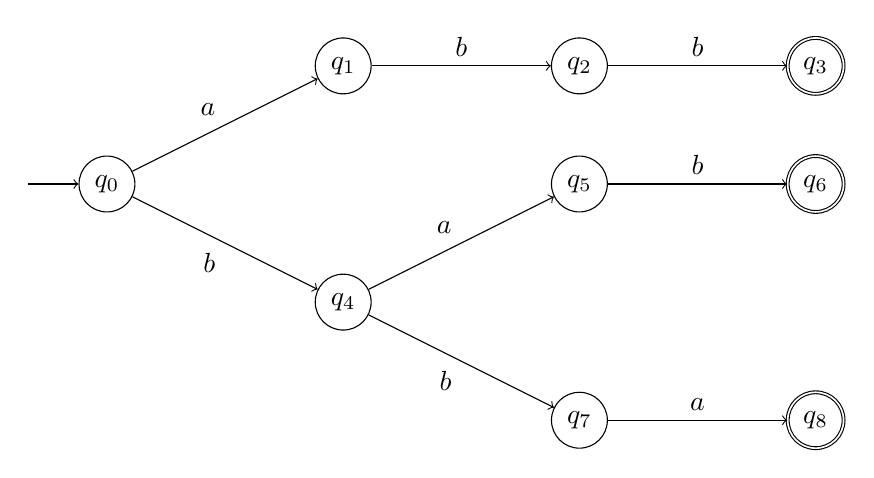
\begin{tikzpicture}
				\node[circle,draw=black, fill=white] (q0) at (0,0) {$q_0$};
				\node[circle,draw=black, fill=white] (q1) at (3,1.5) {$q_1$};
				\node[circle,draw=black, fill=white] (q2) at (6,1.5) {$q_2$};
				\node[circle,draw=black, fill=white,double] (q3) at (9,1.5) {$q_3$};
				\node[circle,draw=black, fill=white] (q4) at (3,-1.5) {$q_4$};
				\node[circle,draw=black, fill=white] (q5) at (6,0) {$q_5$};
				\node[circle,draw=black, fill=white,double] (q6) at (9,0) {$q_6$};
				\node[circle,draw=black, fill=white] (q7) at (6,-3) {$q_7$};
				\node[circle,draw=black, fill=white,double] (q8) at (9,-3) {$q_8$};
				
				\draw[->] (-1,0) -- (q0);
				\draw[->] (q0) to node[midway,above left] {$a$} (q1);
				\draw[->] (q0) to node[midway,below left] {$b$} (q4);
				\draw[->] (q1) to node[midway,above] {$b$} (q2);
				\draw[->] (q2) to node[midway,above] {$b$} (q3);
				\draw[->] (q4) to node[midway,above left] {$a$} (q5);
				\draw[->] (q4) to node[midway,below left] {$b$} (q7);
				\draw[->] (q5) to node[midway,above] {$b$} (q6);
				\draw[->] (q7) to node[midway,above] {$a$} (q8);
			\end{tikzpicture}
		\end{center}
	\end{enumerate}

	\section*{Aufgabe 7.3}
	
	\begin{enumerate}[label=(\alph*)]
		\item $\mathcal{A}=(\{q_0,q_1,q_2,q_3\}\times \{p_0,p_1,p_2,p_3\},\Sigma, (q_0,p_0), \Delta_a,\{q_2,q_3\}\times \{p_3\})$ mit $\Delta_a$
		\begin{center}
			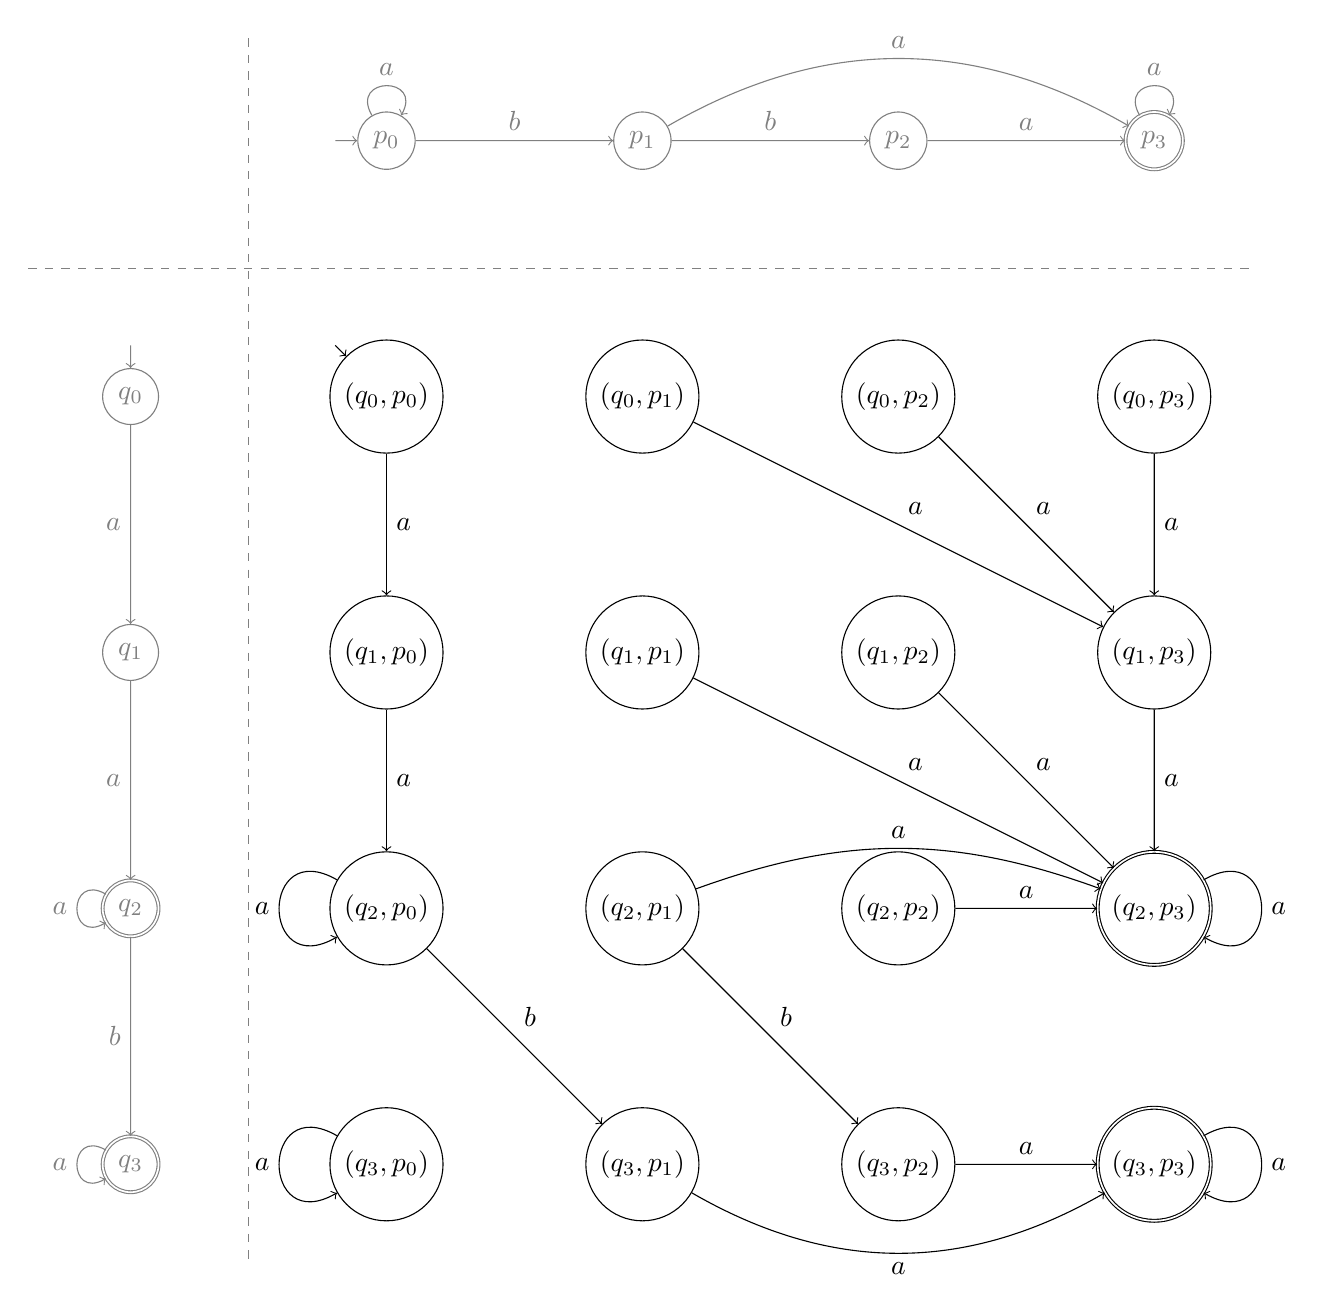
\begin{tikzpicture}[scale=0.65]
			\node[circle,draw=black, fill=white] (q0p0) at (0,0) {$(q_0,p_0)$};
			\node[circle,draw=black, fill=white] (q0p1) at (5,0) {$(q_0,p_1)$};
			\node[circle,draw=black, fill=white] (q0p2) at (10,0) {$(q_0,p_2)$};
			\node[circle,draw=black, fill=white] (q0p3) at (15,0) {$(q_0,p_3)$};
			
			\node[circle,draw=black, fill=white] (q1p0) at (0,-5) {$(q_1,p_0)$};
			\node[circle,draw=black, fill=white] (q1p1) at (5,-5) {$(q_1,p_1)$};
			\node[circle,draw=black, fill=white] (q1p2) at (10,-5) {$(q_1,p_2)$};
			\node[circle,draw=black, fill=white] (q1p3) at (15,-5) {$(q_1,p_3)$};
			
			\node[circle,draw=black, fill=white] (q2p0) at (0,-10) {$(q_2,p_0)$};
			\node[circle,draw=black, fill=white] (q2p1) at (5,-10) {$(q_2,p_1)$};
			\node[circle,draw=black, fill=white] (q2p2) at (10,-10) {$(q_2,p_2)$};
			\node[circle,draw=black, fill=white,double] (q2p3) at (15,-10) {$(q_2,p_3)$};
			
			\node[circle,draw=black, fill=white] (q3p0) at (0,-15) {$(q_3,p_0)$};
			\node[circle,draw=black, fill=white] (q3p1) at (5,-15) {$(q_3,p_1)$};
			\node[circle,draw=black, fill=white] (q3p2) at (10,-15) {$(q_3,p_2)$};
			\node[circle,draw=black, fill=white,double] (q3p3) at (15,-15) {$(q_3,p_3)$};
			
			\node[gray,circle,draw=gray, fill=white] (q0) at (-5,0) {$q_0$};
			\node[gray,circle,draw=gray, fill=white] (q1) at (-5,-5) {$q_1$};
			\node[gray,circle,draw=gray, fill=white,double] (q2) at (-5,-10) {$q_2$};
			\node[gray,circle,draw=gray, fill=white,double] (q3) at (-5,-15) {$q_3$};
			
			\node[gray,circle,draw=gray, fill=white] (p0) at (0,5) {$p_0$};
			\node[gray,circle,draw=gray, fill=white] (p1) at (5,5) {$p_1$};
			\node[gray,circle,draw=gray, fill=white] (p2) at (10,5) {$p_2$};
			\node[gray,circle,draw=gray, fill=white,double] (p3) at (15,5) {$p_3$};
			
			\draw[->] (-1,1) -- (q0p0);
			
			\draw[->] (q0p0) to node[midway,right] {$a$} (q1p0);
			\draw[->] (q1p0) to node[midway,right] {$a$} (q2p0);
			\draw[->] (q2p0) to node[midway,above right] {$b$} (q3p1);
			\draw[->,looseness=4] (q2p0) to[out=150,in=210] node[midway,left] {$a$} (q2p0);
			\draw[->,looseness=4] (q3p0) to[out=150,in=210] node[midway,left] {$a$} (q3p0);
			
			\draw[->] (q0p1) to node[midway,above right] {$a$} (q1p3);
			\draw[->] (q1p1) to node[midway,above right] {$a$} (q2p3);
			\draw[->] (q2p1) to[bend left=20] node[midway,above] {$a$} (q2p3);
			\draw[->] (q2p1) to node[midway,above right] {$b$} (q3p2);
			\draw[->] (q3p1) to[bend right=30] node[midway,below] {$a$} (q3p3);
			
			\draw[->] (q0p2) to node[midway,above right] {$a$} (q1p3);
			\draw[->] (q1p2) to node[midway,above right] {$a$} (q2p3);
			\draw[->] (q2p2) to node[midway,above] {$a$} (q2p3);
			\draw[->] (q3p2) to node[midway,above] {$a$} (q3p3);
			
			\draw[->] (q0p3) to node[midway,right] {$a$} (q1p3);
			\draw[->] (q1p3) to node[midway,right] {$a$} (q2p3);
			\draw[->,looseness=4] (q2p3) to[out=30,in=-30] node[midway,right] {$a$} (q2p3);
			\draw[->,looseness=4] (q3p3) to[out=30,in=-30] node[midway,right] {$a$} (q3p3);
			
			\draw[gray,->] (-5,1) -- (q0);
			\draw[gray,->] (q0) to node[midway,left,gray] {$a$} (q1);
			\draw[gray,->] (q1) to node[midway,left,gray] {$a$} (q2);
			\draw[gray,->] (q2) to node[midway,left,gray] {$b$} (q3);
			\draw[gray,->,looseness=4] (q2) to[out=150,in=210] node[midway,left] {$a$} (q2);
			\draw[gray,->,looseness=4] (q3) to[out=150,in=210] node[midway,left] {$a$} (q3);
			
			\draw[gray,->] (-1,5) -- (p0);
			\draw[gray,->] (p0) to node[midway,above,gray] {$b$} (p1);
			\draw[gray,->] (p1) to node[midway,above,gray] {$b$} (p2);
			\draw[gray,->] (p2) to node[midway,above,gray] {$a$} (p3);
			\draw[gray,->] (p1) to[bend left=30] node[midway,above,gray] {$a$} (p3);
			\draw[gray,->,looseness=4] (p0) to[out=120,in=60] node[midway,above] {$a$} (p0);
			\draw[gray,->,looseness=4] (p3) to[out=120,in=60] node[midway,above] {$a$} (p3);
			
			\draw[gray,dashed] (-7,2.5) -- (17,2.5);
			\draw[gray,dashed] (-2.7,7) -- (-2.7,-17);
			\end{tikzpicture}
		\end{center}
		\item $\mathcal{B}=(\{q_{01},q_1,q_2,q_3\}\cup \{q_0\},\Sigma,q_0,\Delta_b,\{q_0\})$ mit $\Delta_b$
		\begin{center}
			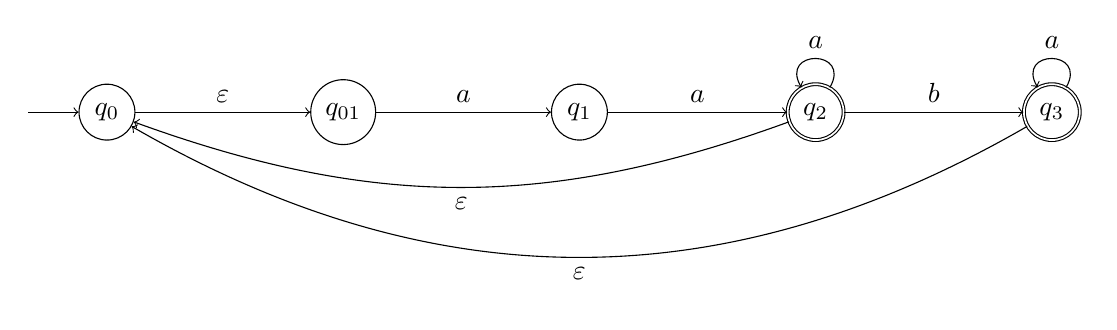
\begin{tikzpicture}
			\node[circle,draw=black, fill=white] (q0) at (0,0) {$q_0$};
			\node[circle,draw=black, fill=white] (q01) at (3,0) {$q_{01}$};
			\node[circle,draw=black, fill=white] (q1) at (6,0) {$q_1$};
			\node[circle,draw=black, fill=white,double] (q2) at (9,0) {$q_2$};
			\node[circle,draw=black, fill=white,double] (q3) at (12,0) {$q_3$};
			
			\draw[->] (-1,0) -- (q0);	
			\draw[->] (q0) to node[midway,above] {$\varepsilon$} (q01);
			\draw[->] (q01) to node[midway,above] {$a$} (q1);
			\draw[->] (q1) to node[midway,above] {$a$} (q2);
			\draw[->] (q2) to node[midway,above] {$b$} (q3);
			\draw[->,looseness=4] (q2) to[out=60,in=120] node[midway,above] {$a$} (q2);
			\draw[->,looseness=4] (q3) to[out=60,in=120] node[midway,above] {$a$} (q3);
			\draw[->] (q2) to[bend left=20] node[midway,below] {$\varepsilon$} (q0);
			\draw[->] (q3) to[bend left=30] node[midway,below] {$\varepsilon$} (q0);
			\end{tikzpicture}
		\end{center}
		Dieser Automat ist noch nicht $\varepsilon$-frei, hier die $\varepsilon$-freie Version:
		\begin{center}
			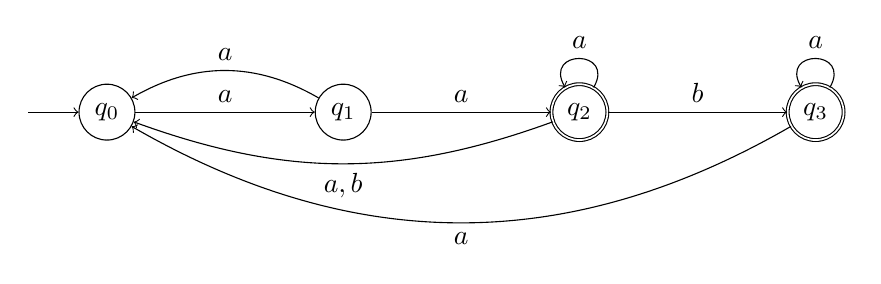
\begin{tikzpicture}
			\node[circle,draw=black, fill=white] (q0) at (0,0) {$q_0$};
			\node[circle,draw=black, fill=white] (q1) at (3,0) {$q_1$};
			\node[circle,draw=black, fill=white,double] (q2) at (6,0) {$q_2$};
			\node[circle,draw=black, fill=white,double] (q3) at (9,0) {$q_3$};
			
			\draw[->] (-1,0) -- (q0);	
			\draw[->] (q0) to node[midway,above] {$a$} (q1);
			\draw[->] (q1) to node[midway,above] {$a$} (q2);
			\draw[->] (q2) to node[midway,above] {$b$} (q3);
			\draw[->,looseness=4] (q2) to[out=60,in=120] node[midway,above] {$a$} (q2);
			\draw[->,looseness=4] (q3) to[out=60,in=120] node[midway,above] {$a$} (q3);
			\draw[->] (q2) to[bend left=20] node[midway,below] {$a,b$} (q0);
			\draw[->] (q3) to[bend left=30] node[midway,below] {$a$} (q0);
			\draw[->] (q1) to[bend right=30] node[midway,above] {$a$} (q0);
			\end{tikzpicture}
		\end{center}
		\item $\mathcal{C}=(\{s_0,s_1,s_2,s_3\}\cup \{t_0,...,t_5\}\cup \{q_0\},\Sigma,q_0,\Delta_c, \{s_3\}\cup \{t_3,t_5\})$ mit $\Delta_c$
		\begin{center}
			\begin{tikzpicture}
			\node[circle,draw=black, fill=white] (q0) at (0,0) {$q_0$};
			
			\node[circle,draw=black, fill=white] (s0) at (3,3) {$s_0$};
			\node[circle,draw=black, fill=white] (s1) at (6,3) {$s_1$};
			\node[circle,draw=black, fill=white] (s2) at (9,4.5) {$s_2$};
			\node[circle,draw=black, fill=white,double] (s3) at (9,1.5) {$s_3$};
			
			\node[circle,draw=black, fill=white] (t0) at (3,-3) {$t_0$};
			\node[circle,draw=black, fill=white] (t1) at (6,-3) {$t_1$};
			\node[circle,draw=black, fill=white] (t2) at (6,-6) {$t_2$};
			\node[circle,draw=black, fill=white,double] (t3) at (9,-3) {$t_3$};
			\node[circle,draw=black, fill=white] (t4) at (12,-3) {$t_4$};
			\node[circle,draw=black, fill=white,double] (t5) at (12,-6) {$t_5$};
			
			\draw[->] (-1,0) -- (q0);
			\draw[->] (q0) to node[midway, above left] {$\varepsilon$} (s0);
			\draw[->] (q0) to node[midway, below left] {$\varepsilon$} (t0);
			
			\draw[->] (s0) to node[midway,above] {$b$} (s1);
			\draw[->] (s1) to node[midway,above left] {$a$} (s2);
			\draw[->] (s2) to node[midway,right] {$a$} (s3);
			\draw[->] (s3) to node[midway,above right] {$b$} (s1);
			\draw[->,looseness=4] (s0) to[out=60,in=120] node[midway,above] {$a$} (s0);
			
			\draw[->] (t0) to node[midway,above] {$a,b$} (t1);
			\draw[->] (t1) to[bend left=30] node[midway,right] {$a$} (t2);
			\draw[->] (t2) to[bend left=30] node[midway,left] {$a$} (t1);
			\draw[->] (t1) to node[midway,above] {$b$} (t3);
			\draw[->] (t3) to node[midway,above] {$b$} (t4);
			\draw[->] (t4) to node[midway,right] {$b$} (t5);
			\draw[->,looseness=4] (t5) to[out=240,in=300] node[midway,below] {$a$} (t5);
			\end{tikzpicture}
		\end{center}
		Dieser Automat ist noch nicht $\varepsilon$-frei, hier die $\varepsilon$-freie Version:
		\begin{center}
			\begin{tikzpicture}
			\node[circle,draw=black, fill=white] (q0) at (0,0) {$q_0$};
			
			\node[circle,draw=black, fill=white] (s0) at (3,3) {$s_0$};
			\node[circle,draw=black, fill=white] (s1) at (6,3) {$s_1$};
			\node[circle,draw=black, fill=white] (s2) at (9,4.5) {$s_2$};
			\node[circle,draw=black, fill=white,double] (s3) at (9,1.5) {$s_3$};
			
			\node[circle,draw=black, fill=white] (t0) at (3,-3) {$t_0$};
			\node[circle,draw=black, fill=white] (t1) at (6,-3) {$t_1$};
			\node[circle,draw=black, fill=white] (t2) at (6,-6) {$t_2$};
			\node[circle,draw=black, fill=white,double] (t3) at (9,-3) {$t_3$};
			\node[circle,draw=black, fill=white] (t4) at (12,-3) {$t_4$};
			\node[circle,draw=black, fill=white,double] (t5) at (12,-6) {$t_5$};
			
			\draw[->] (-1,0) -- (q0);
			\draw[->] (q0) to node[midway, above left] {$a$} (s0);
			\draw[->] (q0) to node[midway, above right] {$a,b$} (t1);
			
			\draw[->] (s0) to node[midway,above] {$b$} (s1);
			\draw[->] (s1) to node[midway,above left] {$a$} (s2);
			\draw[->] (s2) to node[midway,right] {$a$} (s3);
			\draw[->] (s3) to node[midway,above right] {$b$} (s1);
			\draw[->,looseness=4] (s0) to[out=60,in=120] node[midway,above] {$a$} (s0);
			
			\draw[->] (t0) to node[midway,above] {$a,b$} (t1);
			\draw[->] (t1) to[bend left=30] node[midway,right] {$a$} (t2);
			\draw[->] (t2) to[bend left=30] node[midway,left] {$a$} (t1);
			\draw[->] (t1) to node[midway,above] {$b$} (t3);
			\draw[->] (t3) to node[midway,above] {$b$} (t4);
			\draw[->] (t4) to node[midway,right] {$b$} (t5);
			\draw[->,looseness=4] (t5) to[out=240,in=300] node[midway,below] {$a$} (t5);
			\end{tikzpicture}
		\end{center}
		\item $\mathcal{D}=(\{s_0,s_1,s_2,s_3\}\cup \{t_0,...,t_5\},\Sigma,s_0,\Delta_d,\{t_3,t_5\})$ mit $\Delta_d$
		\begin{center}
			\begin{tikzpicture}[scale=0.8]
			\node[circle,draw=black, fill=white] (s0) at (0,0) {$s_0$};
			\node[circle,draw=black, fill=white] (s1) at (3,0) {$s_1$};
			\node[circle,draw=black, fill=white] (s2) at (6,1.5) {$s_2$};
			\node[circle,draw=black, fill=white] (s3) at (6,-1.5) {$s_3$};
			
			\node[circle,draw=black, fill=white] (t0) at (9,0) {$t_0$};
			\node[circle,draw=black, fill=white] (t1) at (12,0) {$t_1$};
			\node[circle,draw=black, fill=white] (t2) at (12,-3) {$t_2$};
			\node[circle,draw=black, fill=white,double] (t3) at (15,0) {$t_3$};
			\node[circle,draw=black, fill=white] (t4) at (18,0) {$t_4$};
			\node[circle,draw=black, fill=white,double] (t5) at (18,-3) {$t_5$};
			
			\draw[->] (-1,0) -- (s0);
			\draw[->] (s0) to node[midway,above] {$b$} (s1);
			\draw[->] (s1) to node[midway,above left] {$a$} (s2);
			\draw[->] (s2) to node[midway,right] {$a$} (s3);
			\draw[->] (s3) to node[midway,above right] {$b$} (s1);
			\draw[->,looseness=4] (s0) to[out=60,in=120] node[midway,above] {$a$} (s0);
			
			\draw[->] (s3) to node[midway, above left] {$\varepsilon$} (t0);
			
			\draw[->] (t0) to node[midway,above] {$a,b$} (t1);
			\draw[->] (t1) to[bend left=30] node[midway,right] {$a$} (t2);
			\draw[->] (t2) to[bend left=30] node[midway,left] {$a$} (t1);
			\draw[->] (t1) to node[midway,above] {$b$} (t3);
			\draw[->] (t3) to node[midway,above] {$b$} (t4);
			\draw[->] (t4) to node[midway,right] {$b$} (t5);
			\draw[->,looseness=4] (t5) to[out=240,in=300] node[midway,below] {$a$} (t5);
			\end{tikzpicture}
		\end{center}
		Dieser Automat ist noch nicht $\varepsilon$-frei, hier die $\varepsilon$-freie Version:
		\begin{center}
			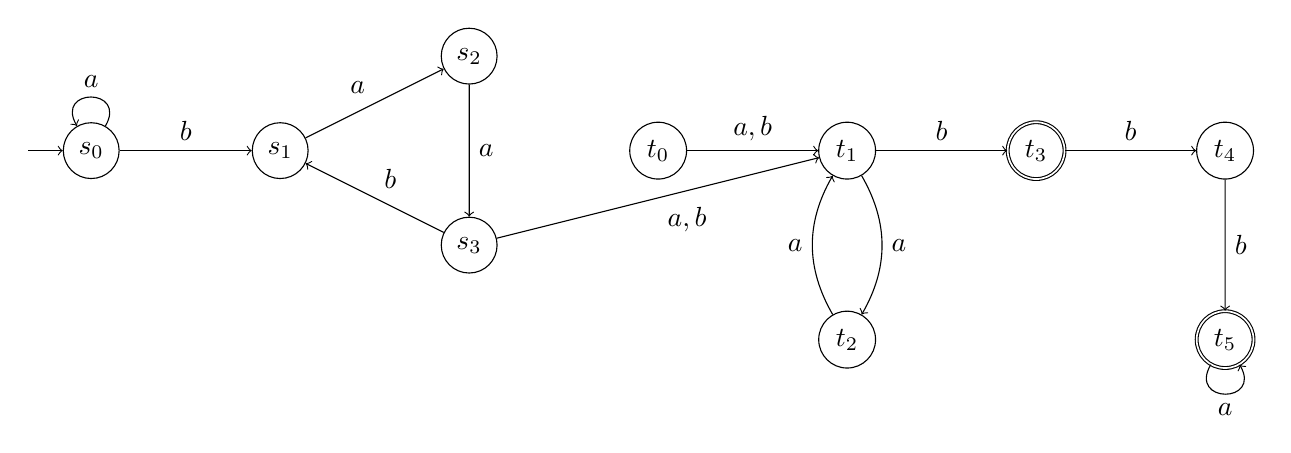
\begin{tikzpicture}[scale=0.8]
			\node[circle,draw=black, fill=white] (s0) at (0,0) {$s_0$};
			\node[circle,draw=black, fill=white] (s1) at (3,0) {$s_1$};
			\node[circle,draw=black, fill=white] (s2) at (6,1.5) {$s_2$};
			\node[circle,draw=black, fill=white] (s3) at (6,-1.5) {$s_3$};
			
			\node[circle,draw=black, fill=white] (t0) at (9,0) {$t_0$};
			\node[circle,draw=black, fill=white] (t1) at (12,0) {$t_1$};
			\node[circle,draw=black, fill=white] (t2) at (12,-3) {$t_2$};
			\node[circle,draw=black, fill=white,double] (t3) at (15,0) {$t_3$};
			\node[circle,draw=black, fill=white] (t4) at (18,0) {$t_4$};
			\node[circle,draw=black, fill=white,double] (t5) at (18,-3) {$t_5$};
			
			\draw[->] (-1,0) -- (s0);
			\draw[->] (s0) to node[midway,above] {$b$} (s1);
			\draw[->] (s1) to node[midway,above left] {$a$} (s2);
			\draw[->] (s2) to node[midway,right] {$a$} (s3);
			\draw[->] (s3) to node[midway,above right] {$b$} (s1);
			\draw[->,looseness=4] (s0) to[out=60,in=120] node[midway,above] {$a$} (s0);
			
			\draw[->] (s3) to node[midway, below right] {$a,b$} (t1);
			
			\draw[->] (t0) to node[midway,above] {$a,b$} (t1);
			\draw[->] (t1) to[bend left=30] node[midway,right] {$a$} (t2);
			\draw[->] (t2) to[bend left=30] node[midway,left] {$a$} (t1);
			\draw[->] (t1) to node[midway,above] {$b$} (t3);
			\draw[->] (t3) to node[midway,above] {$b$} (t4);
			\draw[->] (t4) to node[midway,right] {$b$} (t5);
			\draw[->,looseness=4] (t5) to[out=240,in=300] node[midway,below] {$a$} (t5);
			\end{tikzpicture}
		\end{center}
	\end{enumerate}

\end{document}